\subsection{矩阵规模对 Cache 命中率的影响}

为了分析程序工作集大小对 Cache 命中率的影响，本实验进一步改变矩阵乘法程序中的矩阵规模，分别测试 $N=32$、$N=64$、$N=128$ 三种情况下的 Cache 命中率变化。

矩阵规模会直接影响程序运行时的访存工作集大小。当矩阵规模较小时，主要数据可以较容易地被 Cache 容纳；当矩阵规模增大后，程序访问的数据总量迅速增加，Cache 容量不足时会产生更多容量缺失。

\subsubsection{实验设计}

本组实验固定 Cache 配置，改变矩阵规模。固定参数如下：

\begin{itemize}
    \item Cache 块大小：64B；
    \item 映射方式：4 路组相联；
    \item 替换算法：LRU。
\end{itemize}

变化参数为矩阵规模：

\begin{itemize}
    \item $N=32$；
    \item $N=64$；
    \item $N=128$。
\end{itemize}

对于 int 型矩阵而言，每个元素占 4B。因此，单个 $N \times N$ 矩阵大小为：

\[
MatrixSize = N \times N \times 4B
\]

三个矩阵 $A$、$B$、$C$ 的总数据量为：

\[
WorkingSet = 3 \times N \times N \times 4B
\]

\subsubsection{不同矩阵规模下的工作集大小}

\begin{table}[H]
\centering
\caption{不同矩阵规模下的数据规模}
\begin{tabular}{c|c|c}
\hline
矩阵规模 & 单个矩阵大小 & 三个矩阵总大小 \\
\hline
$N=32$  & 4KB  & 12KB \\
$N=64$  & 16KB & 48KB \\
$N=128$ & 64KB & 192KB \\
\hline
\end{tabular}
\end{table}

从表中可以看出，随着矩阵规模增大，程序的工作集大小呈平方级增长。当 $N=32$ 时，三个矩阵总大小仅为 12KB，较容易被 Cache 容纳；当 $N=128$ 时，三个矩阵总大小达到 192KB，已经明显超过常见的实验 Cache 容量，因此会产生更多容量缺失。

\subsubsection{实验结果}

\begin{table}[H]
\centering
\caption{矩阵规模对 Cache 命中率的影响}
\begin{tabular}{c|c|c|c}
\hline
矩阵规模 & Cache 大小 & 命中率(\%) & Miss 数 \\
\hline
$N=32$  & 32KB & 99.70 &  208 \\
$N=64$  & 32KB & 99.71 & 1566 \\
$N=128$ & 32KB & 49.77  & 2135968 \\
\hline
$N=32$  & 64KB & 99.70 & 208 \\
$N=64$  & 64KB & 99.85 & 1566 \\
$N=128$ & 64KB & 97.27 & 116087 \\
\hline
\end{tabular}
\end{table}

实验数据绘图如下图:
\begin{figure}[H]
     \centering
    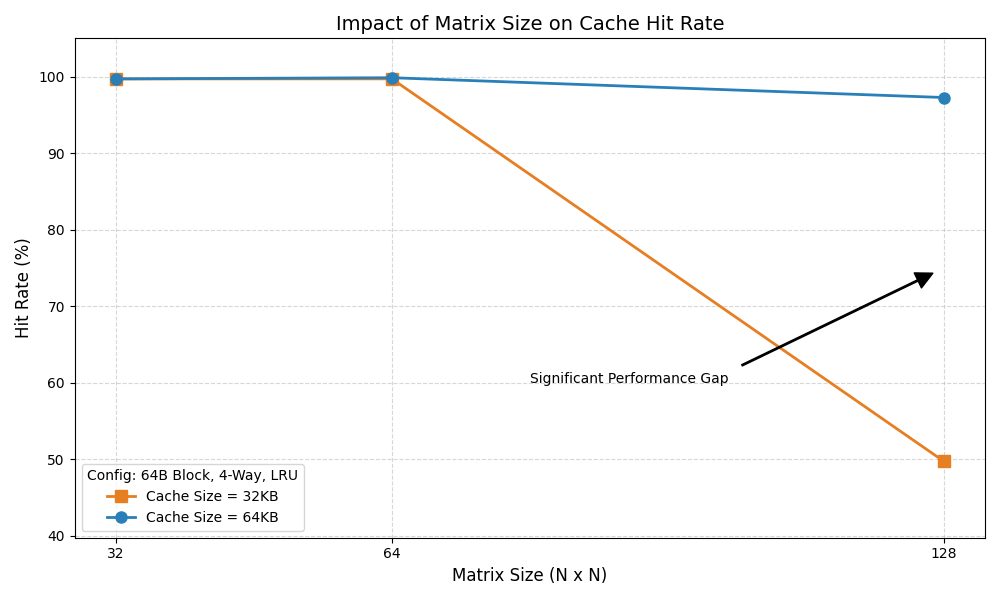
\includegraphics[width = 1\textwidth]{figure/matrix_size_impact.png}
    \caption{矩阵规模对Cache命中率影响}
\end{figure}


\subsubsection{实验现象与分析}

当矩阵规模为 $N=32$ 时，单个矩阵大小为 4KB，三个矩阵总大小为 12KB。在 Cache 容量为 32KB 和 64KB 时，工作集规模均小于 Cache 容量，因此两种配置下的命中率都达到 99.70\%，Miss 数均为 208。这说明在小规模矩阵下，Cache 容量已经足够覆盖主要工作集，继续增大 Cache 容量并不会带来明显收益。

当矩阵规模增大到 $N=64$ 时，单个矩阵大小为 16KB，三个矩阵总大小为 48KB。此时 32KB Cache 已经小于三个矩阵的总大小，但实验结果显示命中率仍然达到 99.71\%；64KB Cache 的命中率为 99.85\%，相比 32KB 仅有小幅提升。这说明虽然总数据量有所增加，但程序在实际运行过程中并不是同时频繁访问全部数据，而是存在一定的活跃工作集和局部性，因此 32KB Cache 仍能维持较高命中率。

当矩阵规模进一步增大到 $N=128$ 时，单个矩阵大小为 64KB，三个矩阵总大小达到 192KB。此时 32KB Cache 已明显无法覆盖主要活跃数据，命中率下降到 49.77\%，Miss 数达到 2135968；而 64KB Cache 的命中率达到 97.27\%，Miss 数降为 116087。由此可见，真正显著的容量差异出现在 $N=128$ 的大规模矩阵场景中。

因此，本组实验的关键现象不是“矩阵规模一增大命中率就立即下降”，而是当矩阵规模增长到使活跃工作集明显超过 Cache 容量时，命中率才会发生显著下降。对于 $N=32$ 和 $N=64$，局部性仍然能够维持较高命中率；对于 $N=128$，32KB Cache 出现明显容量瓶颈，而 64KB Cache 则能显著缓解这一问题。

\subsubsection{实验总结}

通过不同矩阵规模的对比可以看出，矩阵规模会影响程序的工作集大小，但命中率是否显著下降，还取决于活跃工作集与 Cache 容量之间的匹配关系。

在 $N=32$ 和 $N=64$ 时，虽然矩阵规模增大，但程序仍能保持较高命中率，说明此时 Cache 容量和程序局部性仍然能够支撑主要访存需求。而在 $N=128$ 时，32KB Cache 的命中率显著下降到 49.77\%，说明容量不足已经成为主要瓶颈；当 Cache 容量增大到 64KB 后，命中率恢复到 97.27\%，说明较大的 Cache 能够覆盖更多活跃数据，从而显著减少 Miss。

因此，Cache 性能不仅取决于矩阵总数据量，也取决于程序在某一阶段实际反复访问的活跃数据规模。对于矩阵乘法这类数据密集型程序，当矩阵规模较大时，若不通过循环交换、分块等方法改善访存局部性，仅依靠较小容量的 Cache 难以持续保持高命中率。